\chapter{Pruning}
\label{chapter:pruning}

During the search for a complete matching, during which the algorithm only has \textit{partial} matchings, the algorithm will often explore branches of the search tree that will not eventually lead to a homeomorphism. We will call these branches \textit{dead branches}. Exploring an entire dead branch may be costly: its size is exponential\footnote{due to the NP-completeness of node disjoint subgraph homeomorphism} thus exploration costs an exponential amount of time. A solution to this is to implement methods of early detection of such dead branches, i.e. pruning methods. These methods can by nature not detect every dead branch efficiently\footnote{again, because of the NP-completeness of node disjoint subgraph homeomorphism.}. Therefore, there exists a tradeoff between strength, i.e. how many dead branches it can detect, and performance, i.e. how the number of instructions used by pruning scales with the size of the inputs.

%Various pruning methods for subgraph isomorphism exists [refs]. We write bla for subgraph homeomorphism


%if is isomorphism is homeo but homeo not necc iso

%pruning aan de hand van die invariants


%herschrijf pruning methods
Algorithms for subgraph \textit{isomorphism} use various pruning methods, which we will implement for subgraph \textit{homeomorphism}. Subgraph isomorphism is, however, a stricter problem than subgraph homeomorphism. Each subgraph isomorphism mapping is a node disjoint subgraph homeomorphism but not every subgraph homeomorphism is a subgraph isomorphism. Because of this, its pruning methods can filter away some search tree branches that could never result in a subgraph isomorphism, but that could possibly result in a node disjoing subgraph homeomorphism. This means that possibly fewer dead branches can be pruned in the search for subgraph homeomorphisms compared to subgraph isomorphism. In this research, we will experiment with different pruning methods applied to searching subgraph homeomorphisms and draw conclusions about their applicability.

% 
The input of these pruning methods comes down to an assignment of domains (sets of target graph vertices) to variables (source graph vertices). These domains represent the target graph vertex candidates for each source graph vertex in vertex-on-vertex matching. Source graph vertices that are already in the partial matching have a domain of size one: the target graph vertex they have been matched to. The other vertices have domains that can be calculated in different ways (see Section \ref{sec:domain-filtering}). The pruning method then decides whether the algorithm should continue the search in this branch (i.e. do not prune) or whether the algorithm should backtrack. The different methods of deciding this are elaborated in Section \ref{sec:pruningmethods}.

\section{Domain filtering}
\label{sec:domain-filtering}
The goal of domain filtering during a search is to assign a domain of target graph vertices to each source graph vertex such that the following three criteria are satisfied:

\begin{enumerate}
\item \label{li:complete}If at least one homeomorphism can be found from this search branch, then for some homeomorphism that can be found from this search branch with vertex-on-vertex matching $M_V$ it holds that $\forall (s \to t) \in M_V . t \in \mathit{domain}(s)$.
\item \label{li:falsepositives}Each domain assignment contains as few `false positives' as possible, where a false positive is a pair of a source vertex $s$ and a target vertex $t$ such that $t$ is in the domain of variable $s$ and no homeomorphism exists from the current search path in which $s$ is matched to $t$.
\item \label{li:complexity} The process of domain filtering has a computational complexity that is as low as possible.
\end{enumerate}

In this section, we will explore different methods to obtain these domains, each with different tradeoffs between strength (performing better at criterium \ref{li:falsepositives}) and performance (performing better at criterium \ref{li:complexity}).
\subsection{Labels and neighbours}
The weakest and fastest method to obtain domains for some source graph vertex $u$ is by selecting each unmatched target graph vertex $v$ that has compatible labels and has compatible in- and outdegrees:

\begin{minipage}{\textwidth}
\begin{defn}[compability under label constraint] If $M$ is the current partial matching, then:

\[\mathit{compatible}_{\mathit{LABEL}}(u, v) := v \not \in M \land L(u) \subseteq L(v) \land |\mathit{pred}(v)| \geq |\mathit{pred}(u)| \land |\mathit{succ}(v)| \geq |\mathit{succ}(u)|\]

\end{defn}
\end{minipage}

This method satisfies criterium \label{li:complete} since every homeomorphism needs each source graph vertex $u$ to be matched with a target graph vertex $v$ that has at least the same label set as $u$, and the possibility of connecting with each mapped predecessor and successor of $u$. It has a low computational complexity per source-target pair ($O(|L_S|)$).

\subsection{Free neighbours}
A somewhat stronger and somewhat slower method to obtain domains in addition to label filtering is to compare the indegree- and outdegree of each unmatched source graph vertex $u$ to other unmatched source graph vertices to the in- and outdegree of the target graph vertex $v$ to other unmatched target graph vertices. The target graph vertex must have a larger or equal indegree and outdegree compared to the source graph vertex:


\begin{minipage}{\textwidth}
\begin{defn}[compatibility under free neighbours constraint] If $M$ is the current partial matching, then:

$\mathit{compatible}_{\mathit{FN}}(v,u) := \mathit{compatible}_{\mathit{LABEL}}(v,u) \land C_{\mathit{indegree}}(v, u) \land C_{\mathit{outdegree}}(v, u)$

where:

$C_{\mathit{indegree}}(u, v) := |\{v' \in \mathit{pred}(v) .  v' \not \in M\}| \geq |\{u' \in \mathit{pred}(u) . u' \not \in M\}$

$C_{\mathit{outdegree}}(u, v) := |\{v' \in \mathit{succ}(v) . v' \not \in M\}| \geq |\{u' \in \mathit{succ}(u) . u' \not \in M\}$
 
\end{defn}
\end{minipage}

This method satisfies criterium \label{li:complete} since 


\subsection{Reachability of matched vertices}
A strong (and computationally very expensive) method of filtering the domain we will use\footnote{An even stronger method would be to find paths that each have different second vertices and each have different second-last vertices, or even to check that no intermediate vertex is used multiple times (NP-complete). This is, however, out of scope for this research.} for some source graph vertex $u$ and some target graph vertex $v$ in addition to label- indegree and outdegree compability is to check that $v$ can reach the mapped vertices of successors of $u$ and that $v$ can be reached from the mapped vertices of predecessors of $u$, i.e. that candidate paths exist for the upcoming edge-path matching attempts. This pruning method does not check whether a set of paths exist that is vertex disjoint since that is the task of the main algorithm: it merely checks the existence of paths. If no path exists, then no vertex disjoint path exists and pruning is required. An example of a domain filtered by reachability can be found in Figure \ref{fig:reachability-filtered}. Formally:


\begin{minipage}{\textwidth}
\begin{defn}[compatibility under reachability constraint]

If $M$ is the current partial mapping and $P$ is the set of paths in the target graph, then:

$\mathit{compatible}_{\mathit{REACH}}(v,u) := \mathit{compatible}_{\mathit{FN}}(v,u) \land C_{\mathit{inr}}(v, u) \land C_{\mathit{outr}}(v, u)$

where:

\begin{tabular}{lll}
$C_{\mathit{inr}}(u, v) := \forall u' \in (\mathit{pred}(u) \cap M) .  \exists p \in P .$&$\mathit{first}(p)=M(u')$&$\land$\\
&$\mathit{last}(p)=v$&$\land$\\
&\multicolumn{2}{l}{$\not \exists i \in \mathit{intermediate}(p) . i \in M$}
\end{tabular}

\begin{tabular}{lll}
$C_{\mathit{outr}}(u, v) := \forall u' \in (\mathit{succ}(u) \cap M) .  \exists p \in P .$&$\mathit{first}(p)=v$&$\land$\\
&$\mathit{last}(p)=M(u')$&$\land$\\
&\multicolumn{2}{l}{$\not \exists i \in \mathit{intermediate}(p) . i \in M$}
\end{tabular}
\end{defn}
\end{minipage}



\begin{figure}
\centering
\parbox{1.2in}{

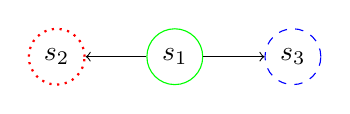
\begin{tikzpicture}

\node[circle, draw=green] at (0,0) (a) {$s_1$};
\node[circle, draw=red, dotted, thick] at (-1.5,0) (b)  {$s_2$};
\node[circle, draw=blue, dashed] at (1.5,0) (c)  {$s_3$};

\draw[->] (a)->(b);
\draw[->] (a)->(c);
\end{tikzpicture}
}
\qquad\qquad
\begin{minipage}{1.2in}%

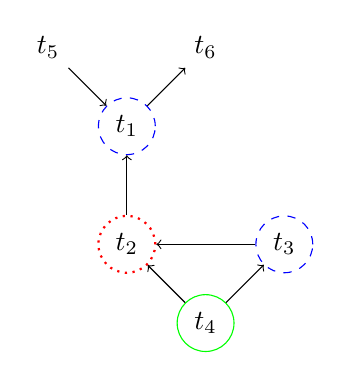
\begin{tikzpicture}
\node[circle, draw=green] at (0,0) (blue) {$t_4$};
\node[circle, draw=red, dotted, thick] at (-1,1) (green) {$t_2$};
\node[circle, draw=blue, dashed] at (1,1) (yellowone) {$t_3$};
\node[circle, draw=blue, dashed] at (-1,2.5) (yellowtwo) {$t_1$};
\node at (-2,3.5) (redone) {$t_5$};
\node at (-0,3.5) (redtwo) {$t_6$};

\draw[->] (blue) -> (green);
\draw[->] (blue) -> (yellowone);
\draw[->] (yellowone) -> (green);
\draw[->] (green) -> (yellowtwo);
\draw[->] (redone) -> (yellowtwo);
\draw[->] (yellowtwo) -> (redtwo);


\end{tikzpicture}
\end{minipage}
\caption{After vertex placements $s_1 \to t_4$ and $s_2 \to t_2$, the domain for vertex $s_3$ would normally be $\{t_1, t_3\}$. However, by checking for reachability from $t_4$ we can reduce this to $\{t_3\}$. The numbers represent the matching order and the circle styles represent labels.}
\label{fig:reachability-filtered}
\end{figure}
\subsection{Reachability of neighbourhood}
In addition to filtering domains based on the current partial matching and the source- and target graph, we can perform domain filtering based on domains that are already computed. If some source graph vertex $s_1$ with domain $D_1$ has an edge to some vertex $s_2$ with domain $D_2$, then for each target graph vertex $t_1 \in D_1$ there must exist a path to some vertex $t_2 \in D_2$. If not, then $t_1$ may be removed from $D_1$. We will call this filtering \textit{level 1 neighbourhood filtering}. If we $D_2$ was itself filtered using level 1 neighbourhood filtering, we call this \textit{level 2 neighbourhood filtering}. Similarly, each additional time the neighbourhood reachability filtered domain is reused in another neighbourhood reachability filtering we consider it of a higher level. When computing domains serially, an appropriate maximum level should be used: using level 2 neighbourhood filtering over level 1 neighbourhood filtering yiels, for example, much more domain reduction and is much less computationally demanding compared to level 20 neighbourhood filtering over level 19 neighbourhood filtering. However, if a cached approach is used (see section TODO), we can perform level $\infty$ neighbourhood filtering using a fixed point algorithm.

\section{Pruning methods}
\label{sec:pruningmethods}
\subsection{ZeroDomain pruning}
%applicable to both isomorphism and homeomorphism
The ZeroDomain pruning method decides to backtrack if and only if one of the domains is empty, i.e. there exists some source graph vertex that cannot be matched with any target graph vertex. A homeomorphism cannot be found in the current search branch as no potential match exists for this source graph vertex. An example of a domain assignment where ZeroDomain prunes the search space is shown in Table \ref{tab:zerodomain}.

\label{sec:emptyDomain}
\begin{table}
\centering
\begin{tabular}{|l|l|}
\hline
\textbf{Source graph vertex} & \textbf{Target graph candidates} \\ \hline
$s_1$                          & $\{t_1, t_3, t_5\}$         \\ \hline
$s_2$                          & $\{t_1, t_2, t_3, t_4\}$       \\ \hline
$s_3$                          & $\{t_2, t_3, t_6\}$      \\ \hline
$s_4$                          & $\emptyset$                      \\ \hline
\end{tabular}
\caption{If the empty domain pruning method detects an empty target graph domain for some source graph vertex, backtracking is initiated. This is the case if the possible target graph candidates are as shown as in this table.}
\label{tab:zerodomain}
\end{table}

\subsection{AllDifferent pruning}
\label{sec:alldifferent}
The AllDifferent constraint specifies that every variable should be able to have a different value. This is the case with some variable having an empty domain (i.e. AllDifferent is stronger than ZeroDomain), but also in other cases. Since a homeomorphism requires such an assignment, the AllDifferent pruning algorithm backtracks in this case. Unfortunately, we could not find an AllDifferent implementation using less than quadratic space. An example of a domain assignment where AllDifferent prunes the search space but ZeroDomain does not is shown in Table \ref{tab:alldifferent}. 

\begin{table}
\centering
\begin{tabular}{|l|l|}
\hline
\textbf{Source graph vertex} & \textbf{Target graph candidates} \\ \hline
$s_1$                          & $\{t_1, t_2, t_3\}$      \\ \hline
$s_2$                          & $\{t_1, t_2\}$              \\ \hline
$s_3$                          & $\{t_2, t_3\}$              \\ \hline
$s_4$                          & $\{t_1, t_3\}$             \\ \hline
\end{tabular}
\caption{In this example, four source graph vertices have a total domain of only three target graph candidates. By the pigeonhole principle, no injective assignment is possible. AllDifferent recognises this and initiates backtracking.}
\label{tab:alldifferent}
\end{table}




\section{When to apply}
When a pruning method has been selected and a strategy to obtain the domains, one must lastly decide when to apply the pruning method.
\subsection{Runtime calculation}
The simplest option is to calculate the domains and run the pruning strategy each time a vertex is selected for usage in a matching. This could be a target graph vertex that is selected as for vertex-on-vertex matching or a target graph vertex that is part of a path in edge-on-path matching. This changes the partial matching and thus the domains. The pruning method then decides to allow it or to disallow it.
\subsection{Caching domains - incremental domain calculation}
Another option is to cache the domain of each variable and update it based on the current partial matching. This saves valuable time but requires quadratic space\footnote{i.e. some constant $c$ exists such that the space required has an upper bound of $c * |V_{target}|^2$} (for each source graph vertex $\in |V_{source}|$ it needs to store a domain of average size $O(|V_{target}|)$). If the reachability pruning method is used, paths need to be cached as well. That is, for each edge $\in E_{source}$ we need to store a path of $O(|V_{target}|)$ vertices.
\subsection{Parallel calculation}
Finally, we can perform the domain filtering and procedure in a seperate CPU thread while the algorithm continues without backtracking. The pruning thread queries the current matching and calculates whether pruning is appropriate for that matching. If it decides that it is not, it requeries the current matching. Otherwise, it will interrupt the main thread and signal it to backtrack until the pruning method does not detect a dead branch anymore. This method cannot perform caching
